\documentclass[conference,10pt]{IEEEtran}
\usepackage{graphicx}
\usepackage{amsmath,amssymb}
\usepackage{booktabs}
\usepackage{array}
\usepackage{url}
\usepackage{xcolor}
\usepackage{microtype}
\usepackage{balance}
\graphicspath{{figures/}}
\newcommand{\sdev}{\mathrm{SD}}
\title{Discretization, Training Budget, and Target-Network Cadence in Tabular Q-Learning and Deep Q-Networks: A Reproducible Gymnasium Study}
\author{\IEEEauthorblockN{[Author name to be confirmed]}\IEEEauthorblockA{Yachay Tech University, Ecuador\\\texttt{email to be added}}}
\begin{document}
\maketitle
\begin{abstract}
The choice between tabular and neural action-value methods depends not only on the size of the observation space but also on discretization, optimization, and training stability. This study implements tabular Q-learning and Deep Q-Networks (DQN) without prebuilt reinforcement-learning agents and evaluates them on CartPole-v1 and Acrobot-v1. We analyze three tabular discretizations (6, 10, and 20 bins per observation dimension), a DQN baseline, two step budgets on CartPole (80,000 and 200,000), and a one-factor-at-a-time sweep of learning rate and target-network update frequency on Acrobot (100,000 steps). Each condition uses three training seeds and a 100-episode greedy final evaluation per seed. At 80,000 steps, 10-bin Q-learning obtained a mean CartPole return of 276.47 versus 91.24 for DQN. In a separately trained 200,000-step follow-up, its mean was 414.69 versus 92.02 for DQN; one of three tabular seeds exceeded the assignment threshold of 475. In Acrobot, DQN with target synchronization every 250 steps achieved $-88.39$ mean return and passed the $-100$ threshold in all three seeds, whereas the baseline obtained $-489.47$. These findings establish strong configuration sensitivity within this implementation, not algorithm-wide superiority. We discuss unequal exploration schedules across step budgets, small-sample uncertainty, and limits of target-network ablation.
\end{abstract}
\begin{IEEEkeywords}
Reinforcement learning, Q-learning, deep Q-network, discretization, target network, reproducibility, Gymnasium.
\end{IEEEkeywords}

\section{Introduction}
Reinforcement learning (RL) uses interactions with an environment to learn behavior that maximizes cumulative reward \cite{Sutton2018}. Classical tabular Q-learning stores a separate estimate for each state--action pair. Deep Q-Networks (DQN) replace this table with a parameterized value function, allowing generalization among related continuous observations \cite{Mnih2015}. However, improved representational capacity does not imply reliable learning in every task: bootstrapped targets, stochastic optimization, correlated observations, and delayed rewards can introduce substantial instability.

For an observation vector with only a few continuous coordinates, discretization may remain a practical alternative to neural approximation. Its computational simplicity comes at the cost of state aliasing and a rapidly growing state space. Conversely, DQN avoids an explicit state grid but trades it for dependence on optimizer settings, experience replay, and a periodically synchronized target network. A rigorous comparison must therefore distinguish representation, training budget, and evaluation protocol rather than merely report a successful episode.

We investigate three questions: \emph{(RQ1)} How does tabular discretization affect CartPole performance at a fixed interaction budget? \emph{(RQ2)} How do independently trained 80,000- and 200,000-step configurations compare, acknowledging that the exploration schedule also scales with budget? \emph{(RQ3)} How sensitive is DQN on Acrobot to learning rate, target update frequency, and removal of the target network? The goal is a documented educational experiment with auditable negative as well as positive outcomes, not a claim of state-of-the-art performance.

Our contributions are: (i) self-contained Python/PyTorch implementations with episode-level logging; (ii) a matched-step CartPole comparison across three discretization granularities and DQN; (iii) an Acrobot sensitivity study with a controlled no-target ablation; and (iv) an analysis of uncertainty, evaluation leakage risks, continuous-action suitability, and the interpretation of failure cases. All reported numerical results were recalculated from the supplied experiment logs rather than estimated from plotted curves.

\section{Problem and Algorithmic Background}
\subsection{Environment selection and suitability}
A Markov decision process is represented by $(\mathcal S,\mathcal A,P,r,\gamma)$, where $\mathcal S$ is the state space, $\mathcal A$ is the action space, $P$ is the transition law, $r$ is the reward function, and $\gamma$ discounts future rewards. For action-value methods, the critical distinction is between observation and action dimensionality. CartPole-v1 exposes four continuous observations and two discrete actions; Acrobot-v1 uses six continuous observations and three discrete actions \cite{GymnasiumDocs}. These tasks admit standard DQN because its output layer contains one Q-value per discrete action. Tabular Q-learning requires quantization of its continuous observations.

The assignment defines successful performance as mean return at least 475 for CartPole and at least $-100$ for Acrobot over 100 episodes. These are the \emph{assignment thresholds}; they should not be confused with different thresholds that may appear in the installed Gymnasium documentation. CartPole episodes last at most 500 steps, and Acrobot penalties can yield $-500$ when no goal is reached within the horizon.

\subsection{Tabular Q-learning and quantization}
For a discretized observation $\bar{s}$, the off-policy temporal-difference update is
\begin{equation}
\begin{aligned}
Q(\bar s,a)\leftarrow{}&Q(\bar s,a)+\alpha\bigl[r+\gamma(1-d)\\
&\quad\max_{a'}Q(\bar s',a')-Q(\bar s,a)\bigr],
\end{aligned}\label{eq:tabular}
\end{equation}
where $d=1$ only on a genuine terminated transition, $\alpha=0.15$ and $\gamma=0.99$. The implementation uses $b\in\{6,10,20\}$ equal-width bins in each of the four CartPole observation dimensions. The resulting state counts are $b^4=1,296$, $10,000$, and $160,000$; multiplying by two actions gives $2,592$, $20,000$, and $320,000$ Q-values, respectively. With float32 storage, the dense tables require approximately 10.4~kB, 80~kB, and 1.28~MB, excluding array overhead.

The binning range is engineered around the task's relevant region: cart position $[-2.4,2.4]$, cart velocity $[-3,3]$, pole angle $[-0.20944,0.20944]$ radians, and angular velocity $[-3.5,3.5]$. Values beyond these intervals map to extreme bins. This saturating encoding introduces aliasing and must not be mistaken for a discretization with universally optimal boundaries. When $b$ is too small, distinct physical states merge; when $b$ is large, observed transitions may cover only a small fraction of state--action pairs.

\subsection{Deep Q-learning and stabilization}
The DQN function $Q_\theta(s,a)$ is a two-hidden-layer multilayer perceptron with 128 ReLU units per layer. Input dimensions are 4 for CartPole and 6 for Acrobot; the output has 2 or 3 units, one per action. For sampled transition $(s,a,r,s',d)$, vanilla DQN minimizes Huber loss against the fixed-target bootstrap
\begin{equation}
\label{eq:dqn}
y=r+\gamma(1-d)\max_{a'}Q_{\theta^-}(s',a'),
\end{equation}
where $\theta^-$ denotes the target-network parameters. We use Adam, replay capacity 50,000, minibatches of 64, learning beginning at 1,000 environment steps, optimization every four environment steps, and gradient-norm clipping at 10. The baseline target network synchronizes every 1,000 environment steps. The replay buffer samples with replacement and is seeded separately for each run.

Training uses $\epsilon$-greedy behavior while evaluation always uses $\epsilon=0$. The terminal bootstrap mask is based on \texttt{terminated}, whereas an episode ends on \texttt{terminated OR truncated}. This avoids treating a time-limit cutoff as a physical terminal state. In the no-target ablation, next-state values are evaluated using the online network under \texttt{no\_grad}, while replay, network shape, and other training parameters remain unchanged. Because the baseline also fails in most runs, this ablation alone does not identify the target network's necessity across all possible settings.

\section{Experimental Protocol and Reproducibility}
\subsection{Run matrix and fixed evaluation}
We executed 42 full training runs: 12 CartPole runs at 80,000 steps, 12 separate CartPole runs at 200,000 steps, and 18 Acrobot runs at 100,000 steps, totaling 5.16 million training interactions. Each configuration used seeds $\{11,22,33\}$. The 80,000-step CartPole experiment was the initial study; the 200,000-step experiment was a follow-up prompted by the initial underperformance, rather than an a priori independent replication.

The CartPole conditions are tabular 6, 10, and 20 bins and DQN (learning rate $10^{-3}$). The Acrobot sweep is one-factor-at-a-time (OFAT): learning rates $\{0.00025,0.0005,0.001\}$ with target update every 1,000 steps, and target update intervals $\{250,1000,4000\}$ with learning rate $0.0005$. A sixth Acrobot condition removes the target network at the default learning rate and otherwise unchanged settings. Acrobot's $\epsilon$ falls linearly from 1.0 to 0.10 over 80\% of training; CartPole's falls from 1.0 to 0.05 over 70\%.

Every 10,000 training steps, ten greedy episodes are evaluated on a separate environment with reproducible episode seeds. A separate 100-episode final greedy evaluation uses an offset seed range, disjoint from checkpoint seeds. The training-step budget excludes evaluation interactions, but measured wall-clock time includes them. We aggregate the \emph{per-seed} final evaluation means and report their mean and sample standard deviation; the 100 episodes inside each seed do not constitute 100 independent training replications. A threshold is counted as met only if a seed's 100-episode final mean satisfies the assignment criterion. Checkpoint threshold crossings, if shown, remain exploratory.

Training was performed on Windows 11 with Python 3.12.7, Gymnasium 1.4.0, PyTorch 2.15.0 (CPU build), NumPy 2.5.4, and an Intel x86 processor exposing 12 logical CPUs. The DQN code explicitly sets one PyTorch CPU thread. Each run directory stores a JSON configuration, raw training episodes, checkpoint evaluations, final episode-level returns, a summary, and saved policy weights. The result figures can be regenerated directly from logged CSV files. Seeds improve comparability, but do not promise bitwise reproducibility across environments or hardware.

\subsection{Interpretive limits of the follow-up budget}
The 200,000-step runs were initialized from scratch and did not continue the 80,000-step model weights. Moreover, the $\epsilon$-decay schedule is proportional to the chosen training budget, so a run with more steps also explores for longer. Thus, a difference between the 80,000- and 200,000-step conditions reflects a \emph{joint change in budget and exploration schedule}; it is not an isolated treatment effect of environment steps. All algorithms within each CartPole budget share the same step count. This within-budget fairness does not eliminate differences in update frequency, action selection, or wall-clock cost across algorithm families.

\section{Results}
\subsection{CartPole: initial 80,000-step comparison}
Table~\ref{tab:cart} reports the per-seed means of 100-episode holdout returns, aggregated across three seeds. At 80,000 steps, the 10-bin tabular variant produced $276.47\pm101.51$ (mean $\pm$ sample SD), exceeding 6 bins ($205.32\pm40.40$), 20 bins ($139.36\pm19.60$), and DQN ($91.24\pm26.31$). No training seed met the assignment threshold of 475 at the final holdout evaluation. Q-learning's ranking is consistent with a discretization tradeoff at these settings, but the study varies only three choices of uniform bin count; the shape and limits of the discretizer were not independently tuned.

\begin{table}[t]
\caption{CartPole final holdout performance: mean $\pm$ SD across three training seeds (100 greedy episodes per seed).}
\label{tab:cart}
\centering
\footnotesize
\setlength{\tabcolsep}{4pt}
\begin{tabular}{lcc}
\toprule
Variant & 80k steps & 200k steps \\
\midrule
Tabular 6 bins & $205.32\pm40.40$ & $168.78\pm13.10$ \\
Tabular 10 bins & $276.47\pm101.51$ & $414.69\pm59.48$ \\
Tabular 20 bins & $139.36\pm19.60$ & $229.46\pm79.63$ \\
DQN baseline & $91.24\pm26.31$ & $92.02\pm3.25$ \\
\midrule
Threshold met, 10-bin & 0/3 seeds & 1/3 seeds \\
\bottomrule
\end{tabular}
\end{table}

\begin{figure}[t]
\centering
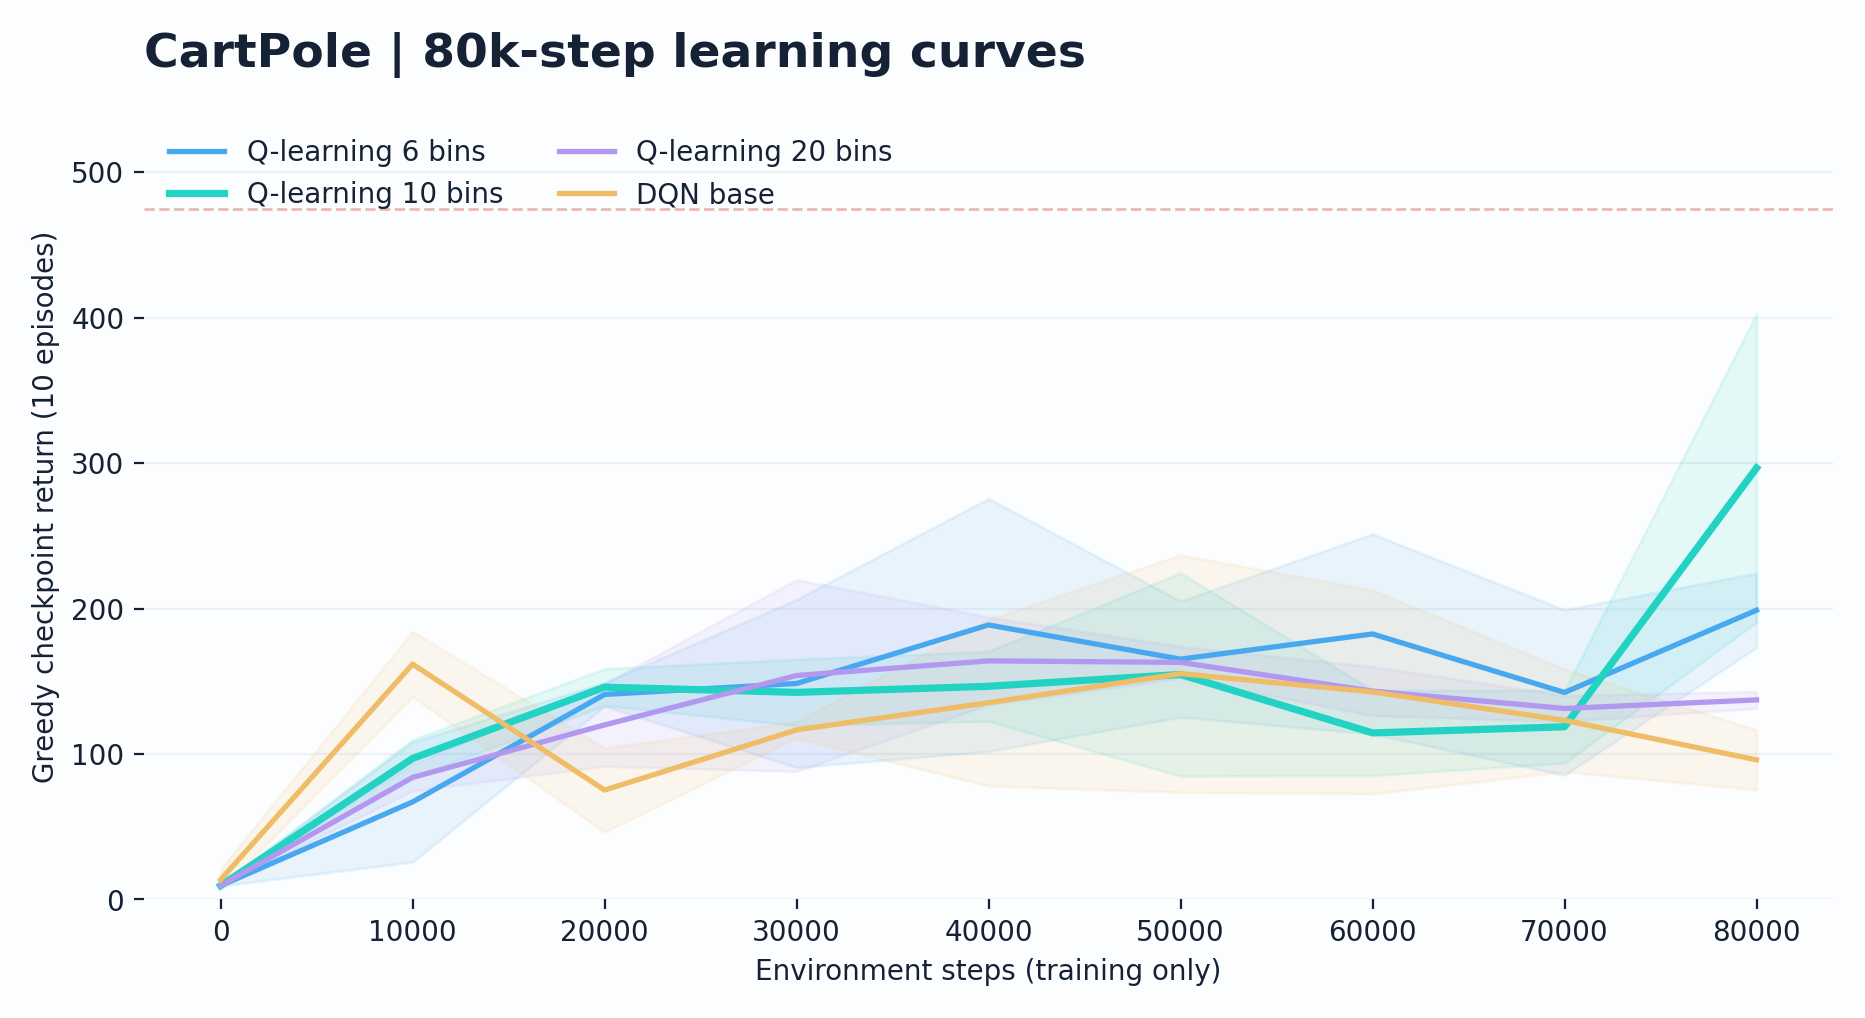
\includegraphics[width=\columnwidth]{tier1_curves_light.png}
\caption{CartPole learning curves at 80,000 training steps: mean and shaded $\pm1$ SD across three training seeds at each ten-episode greedy checkpoint. The dashed line marks the course threshold (475). Curves are descriptive, not 100-episode final evaluations.}
\label{fig:cart80}
\end{figure}

The learning curves in Fig.~\ref{fig:cart80} further distinguish transient checkpoint performance from final holdout performance. A favorable checkpoint is insufficient to establish sustained success: the final evaluation uses a different seed range and ten times more episodes per training seed. Tabular 10 bins exhibited substantial between-seed spread, which is relevant when comparing algorithms from only three random initializations.

\subsection{CartPole: exploratory 200,000-step follow-up}
The follow-up produced $414.69\pm59.48$ for 10-bin Q-learning versus $92.02\pm3.25$ for DQN. The three tabular 10-bin final means were 369.28, 392.78, and 482.02, respectively: only seed 33 exceeded the prescribed 475 cutoff. Although the mean is substantially larger than at 80,000 steps, the follow-up cannot separate additional environment interaction from the longer exploration decay. DQN's reported mean did not meaningfully change within the observed configurations. The 6-bin variant performed worse in the follow-up, while 20 bins improved, showing that a larger training budget is not guaranteed to benefit every tested representation.

\begin{figure}[t]
\centering
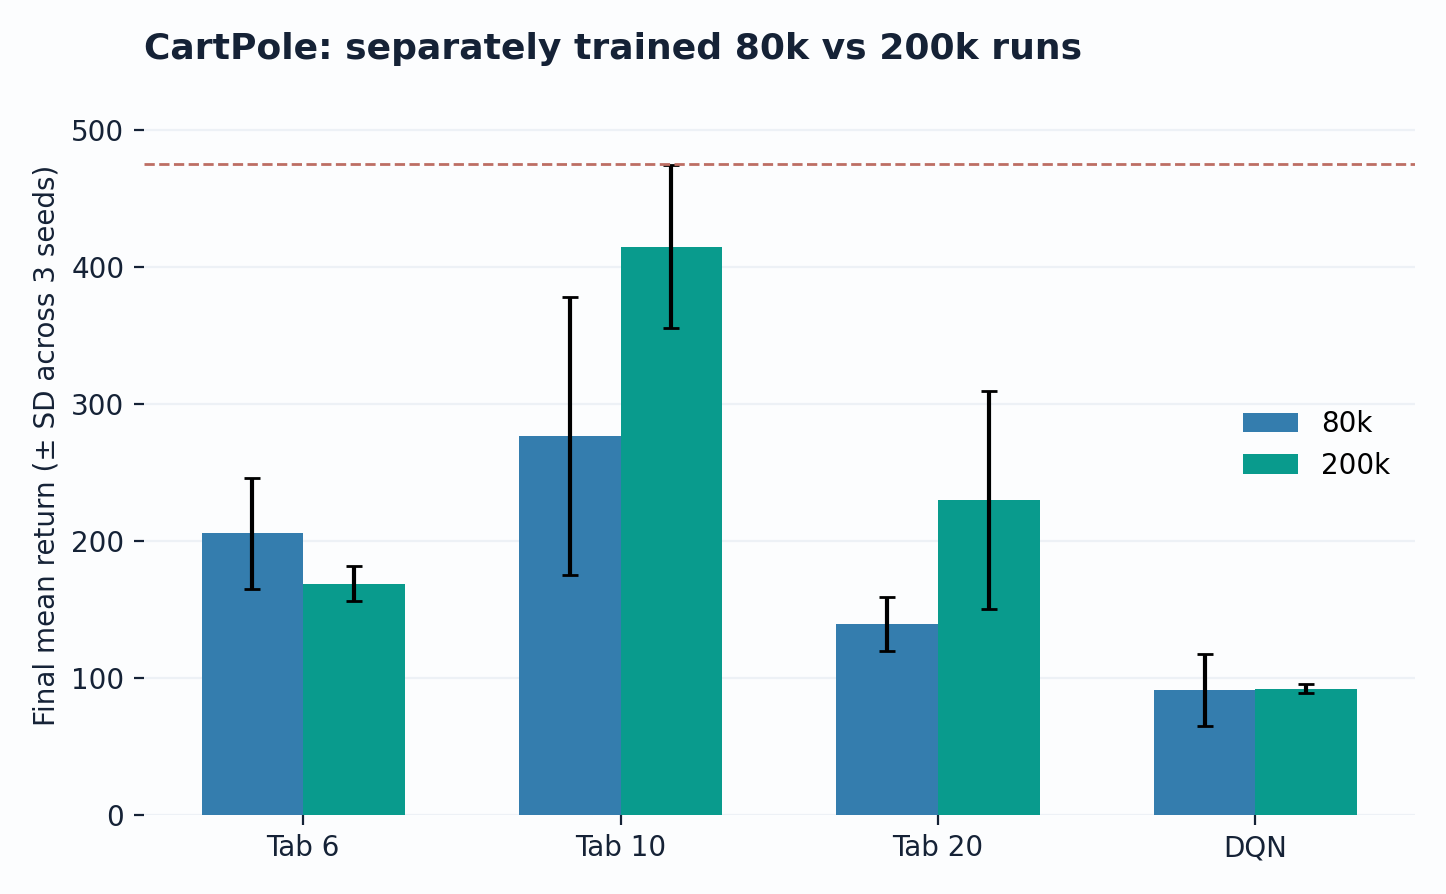
\includegraphics[width=\columnwidth]{paper_cartpole_budget.png}
\caption{Final CartPole performance under two \emph{separately trained} budgets. Bars depict across-seed means with $\pm1$ SD (three seeds each). Longer budgets also stretch $\epsilon$-greedy decay; this plot is not a controlled continuation of trained policies.}
\label{fig:budget}
\end{figure}

The final average of the 10-bin variant remains below 475 even though a single seed passes. Its performance distribution therefore supports a qualified result: the tested configuration \emph{can} meet the threshold under a favorable seed, but reliable attainment across independent runs has not been established. It would be incorrect to report the whole CartPole experiment as solved simply because one of three replications succeeded.

\subsection{Acrobot: hyperparameters and target-network ablation}
Table~\ref{tab:acro} summarizes all six Acrobot conditions after 100,000 training steps. The standout result is target synchronization every 250 steps: the mean was $-88.39\pm5.69$, and all three seeds passed the $-100$ assignment threshold (individual means $-93.76$, $-88.98$, and $-82.42$). The baseline interval of 1,000 steps achieved $-489.47\pm18.23$; the 4,000-step interval and no-target ablation both remained at $-500.00$ for all three seeds. With target update fixed at 1,000, learning rate $0.001$ gave $-372.76\pm220.39$, driven mainly by one seed ($-118.27$), while other seeds returned $-500$. Learning rate $0.00025$ remained at $-500$ throughout its final evaluations.

\begin{table}[t]
\caption{Acrobot final holdout performance at 100k steps ($n=3$ seeds). Higher (less negative) return is better.}
\label{tab:acro}
\centering
\footnotesize
\setlength{\tabcolsep}{3.5pt}
\begin{tabular}{lcc}
\toprule
Configuration & Return: mean $\pm$ SD & Passed \\
\midrule
DQN base (target 1000) & $-489.47\pm18.23$ & 0/3 \\
LR $0.00025$ & $-500.00\pm0.00$ & 0/3 \\
LR $0.001$ & $-372.76\pm220.39$ & 0/3 \\
\textbf{Target 250} & $\mathbf{-88.39\pm5.69}$ & \textbf{3/3} \\
Target 4000 & $-500.00\pm0.00$ & 0/3 \\
No target network & $-500.00\pm0.00$ & 0/3 \\
\bottomrule
\end{tabular}
\end{table}

\begin{figure}[t]
\centering
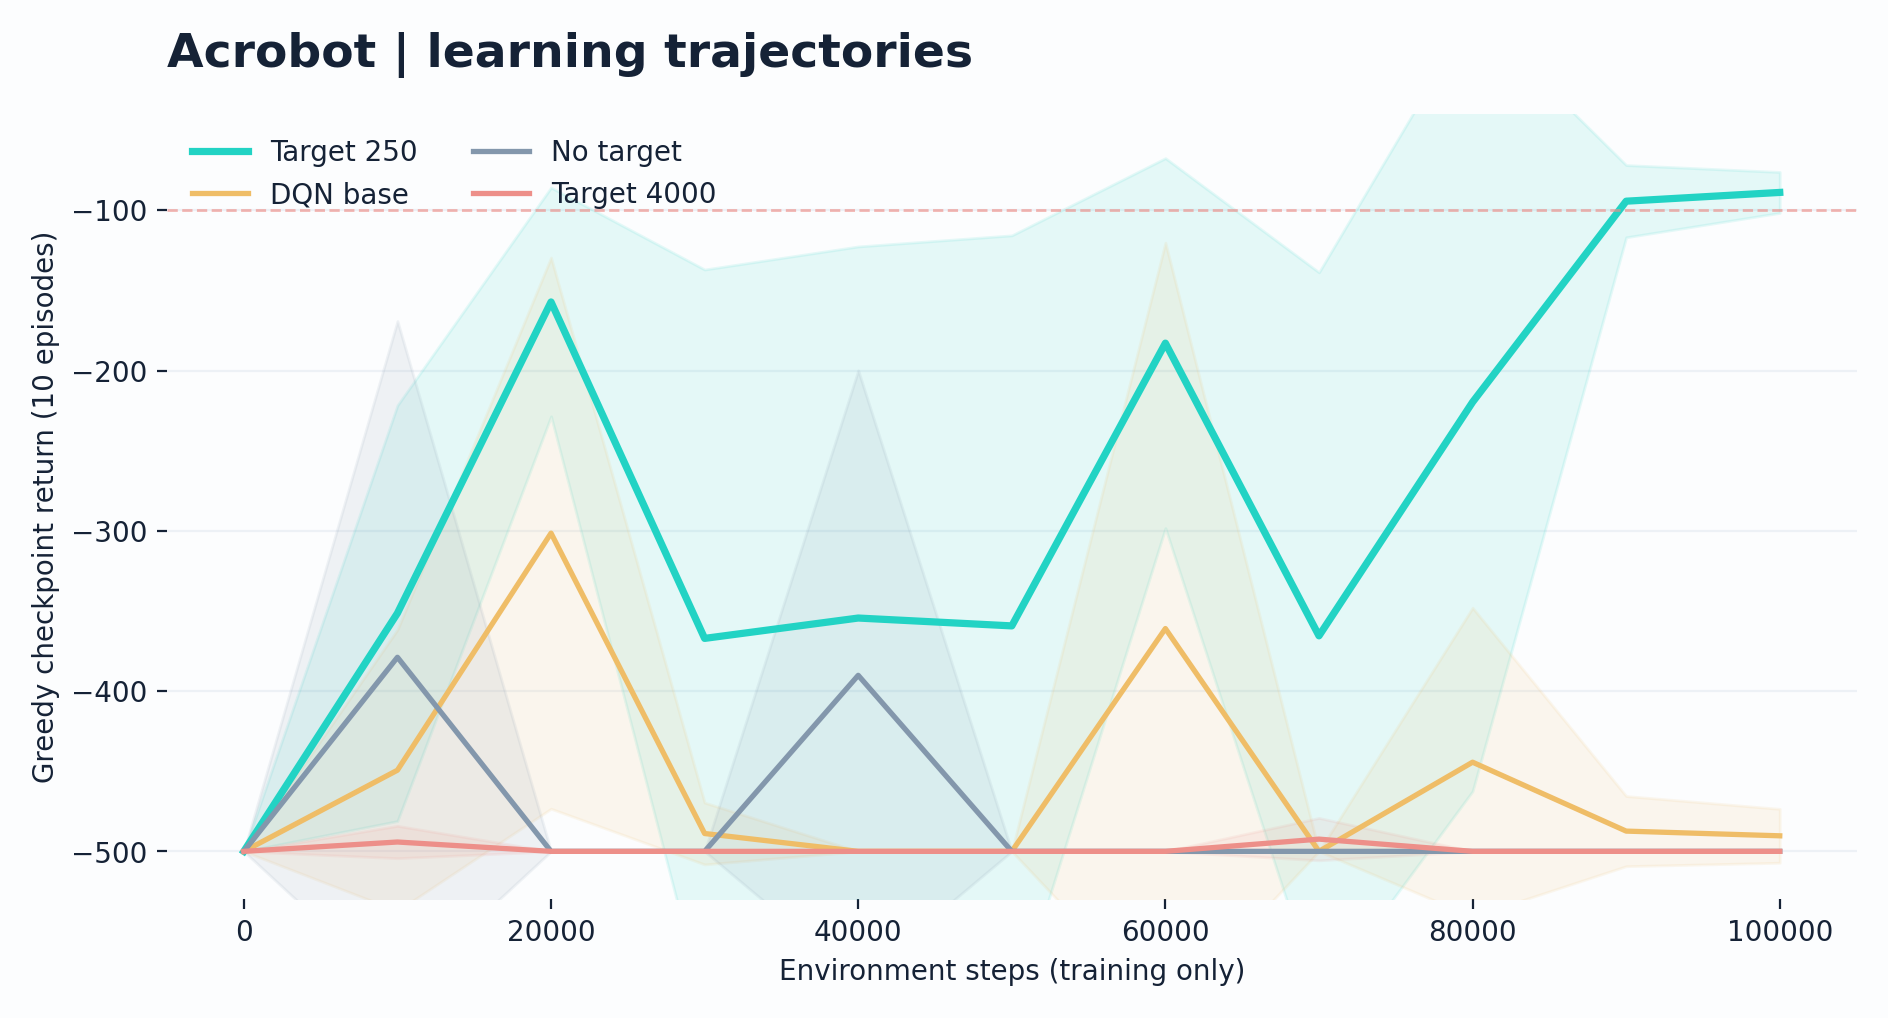
\includegraphics[width=\columnwidth]{tier2_curves_light.png}
\caption{Acrobot checkpoint trajectories (ten greedy episodes/checkpoint) for the baseline, target-250, target-4000, and no-target conditions. Shading indicates $\pm1$ SD across seeds; the line at $-100$ is the course criterion.}
\label{fig:acrocurves}
\end{figure}

The difference of about 401.09 return points between target-250 and baseline is large in this finite sweep, yet it should be interpreted descriptively. The sample size is three training seeds, the tests were not repeated across architectures or environments, and no correction was made for selecting the strongest setting from a suite of alternatives. Critically, the ablation does \emph{not} by itself show a positive effect of merely having a target network: the no-target and target-1000 variants both failed. The combination of a target network \emph{and its update cadence} is the observed distinguishing factor, and a mechanistic conclusion would require a factorial study or additional update schedules.

Checkpoint paths reveal a further nuance: at least some configurations temporarily crossed the threshold before the final evaluation fell short. For example, a baseline Acrobot seed registered an exploratory checkpoint crossing at 60,000 steps but finished with a 100-episode mean of $-468.42$. The trained policy's measured outcome at a particular checkpoint therefore cannot be substituted for a final repeatable success claim.

\section{Within-Seed Contrasts and Diagnostic Evidence}
\subsection{Matched random-seed contrasts}
Although each condition was initialized from three separate random seeds, reusing the same seed identifiers across alternatives allows an exploratory within-seed comparison. Table~\ref{tab:paired} shows the difference between the two policies evaluated under the same nominal training seed. The contrast is descriptive: fixed seed identifiers do not hold training trajectories constant when different epsilon schedules or agents generate different actions, and our sample of three seeds does not support a reliable population-level significance test.

\begin{table}[t]
\caption{Within-seed final-return differences (positive favors the first method). CartPole contrasts compare 10-bin Q-learning minus DQN; Acrobot compares target-250 minus base DQN.}
\label{tab:paired}
\centering\footnotesize\setlength{\tabcolsep}{4pt}
\begin{tabular}{rccc}
\toprule
Seed & CartPole 80k & CartPole 200k & Acrobot 100k \\
\midrule
11 & 185.91 & 274.65 & 406.24 \\
22 & 269.53 & 299.73 & 411.02 \\
33 & 100.26 & 393.64 & 386.00 \\
\midrule
Mean & 185.23 & 322.67 & 401.09 \\
\bottomrule
\end{tabular}
\end{table}

In CartPole, the 10-bin model outperformed the configured DQN for all three seed identifiers at both budgets. The between-seed range of this paired advantage is still wide, particularly in the 80,000-step experiment (100.26 to 269.53). The effect is therefore practically conspicuous but not sufficient evidence that discretized Q-learning dominates DQN in general. The Acrobot target-250 advantage was positive for each matched seed, but because target-250 was the best among several examined update intervals, any confirmatory study should avoid treating this result as an unbiased estimate of a universally optimal target cadence.

\subsection{Three distinct notions of success}
A learned policy can have a favorable training return without successful deployment, a single checkpoint may exceed an evaluation threshold without a corresponding final holdout result, and one training seed may succeed without robust performance across seeds. These are different measurement units. The reported \emph{training returns} are collected under a nonzero exploration probability and therefore measure the behavior policy, not exclusively the final greedy policy. The checkpoint curves are based on ten greedy evaluation episodes and provide coarse temporal diagnostics. The 100-episode holdout is the primary outcome used for the course's success criterion. We never substitute one unit for another.

A concrete example appears in the 200,000-step CartPole follow-up: 10-bin Q-learning crossed 475 in at least one checkpoint for each of the three seeds (at 170k, 140k, and 160k steps), yet only seed 33 remained above 475 on the final 100-episode holdout. Similarly, Acrobot baseline seed 33 crossed the threshold at a checkpoint around step 60k but ended at $-468.42$ on the final test. These patterns are consistent with transient policy quality and/or evaluation noise; the logs alone do not distinguish policy drift from stochastic episode selection. To do so would require repeated independent evaluation episodes at each checkpoint and potentially checkpointed model weights, which were not retained for every intermediate training step.

\begin{figure}[t]
\centering
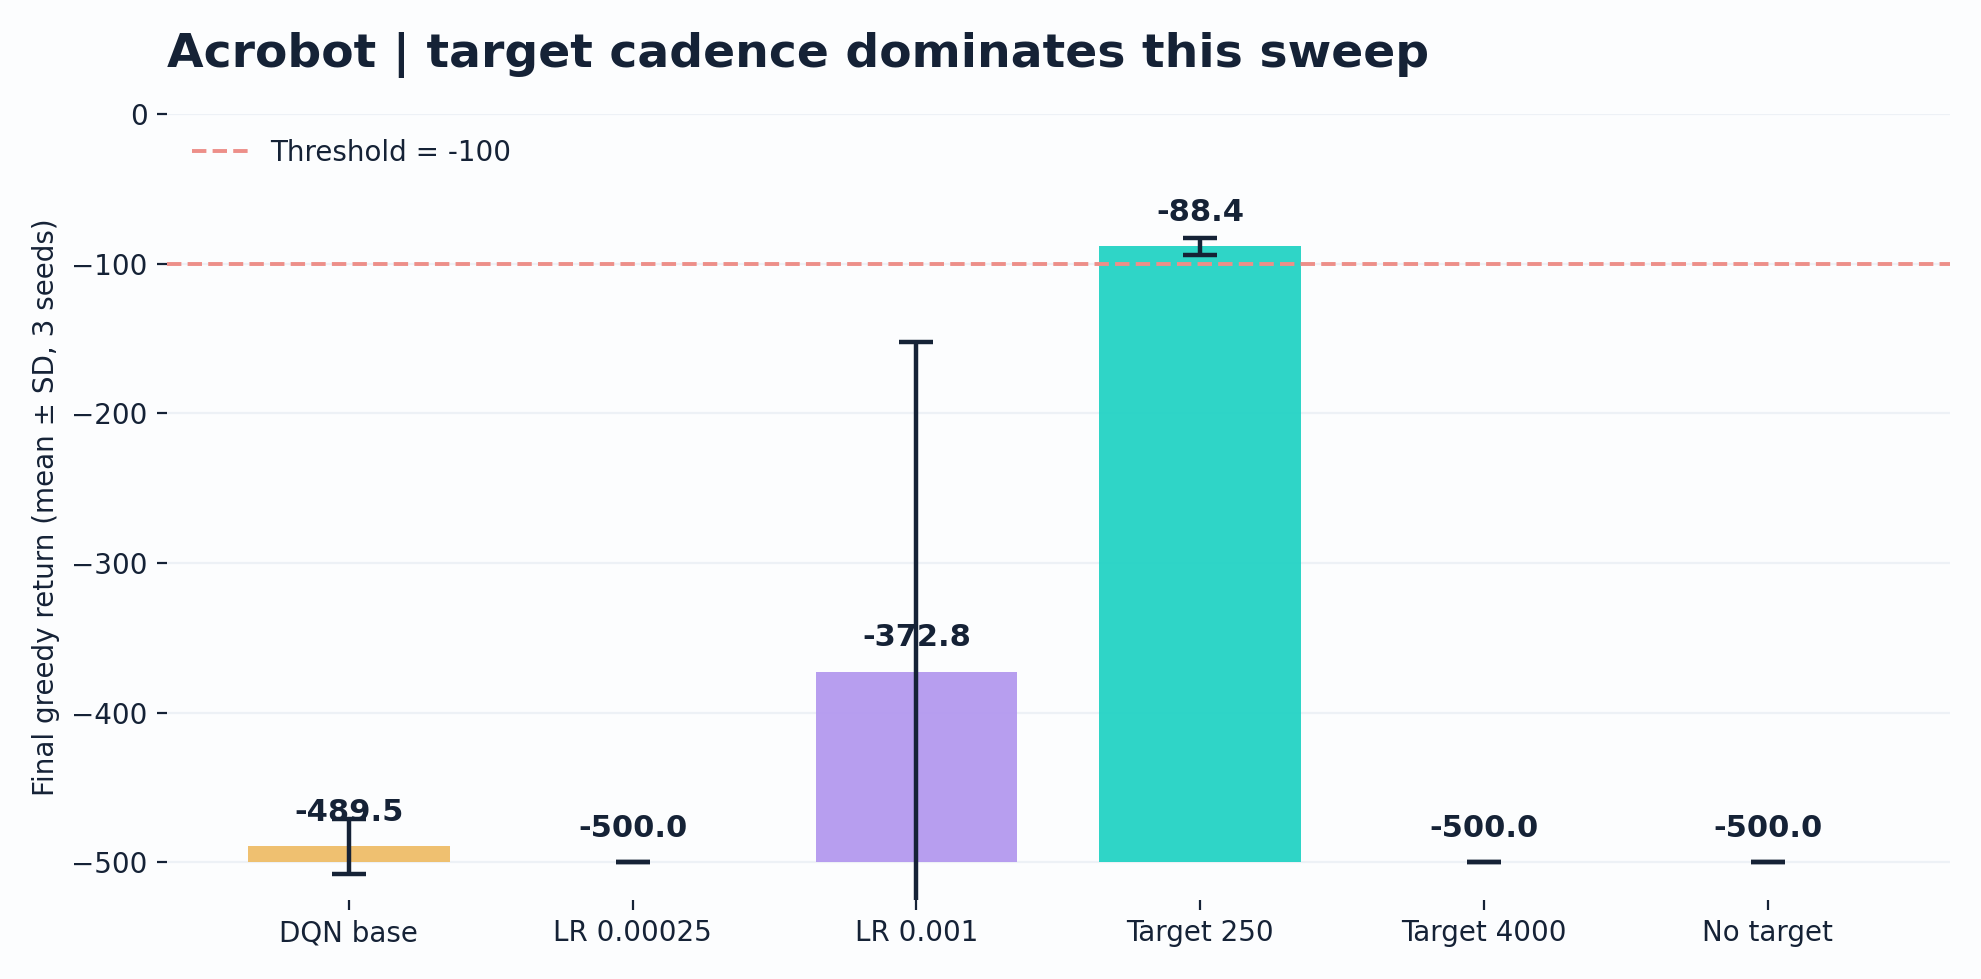
\includegraphics[width=\columnwidth]{tier2_bars_light.png}
\caption{Acrobot final-return means and sample SDs across three training seeds. At the $-500$ return floor, symmetric error bars are uninformative; the large variation of LR 0.001 also reflects seed dependence.}
\label{fig:acrofinal}
\end{figure}

\subsection{What a failed configuration does and does not show}
Several Acrobot variants consistently returned $-500$, the nominal time-limit floor for episodes in which the swing-up objective is not reached. This tells us the trained greedy policy did not achieve the task within the evaluation horizon, but it does not by itself reveal whether the network learned useful intermediate control behaviors. Aggregate rewards may conceal small improvements in state visitation or progress toward the target. The appropriate conclusion is a \emph{failure to reach the defined return objective}, not proof of no learning whatsoever.

For the no-target ablation, the training source confirms that the replay buffer and optimizer remain active and that the online network supplies the bootstrap values. Since baseline synchronization every 1,000 steps also failed, the comparison of these two conditions has little discriminatory power about the binary presence or absence of target stabilization. The stronger evidence is the variation \emph{among target-network configurations}, in which the 250-step interval succeeds and slower intervals do not. A subsequent factorial design would cross update interval with learning rate and repeat the best conditions over more seeds. This would reduce dependence on a single selected hyperparameter schedule.

\subsection{Traceability and code-level checks}
The evidence trail for any plotted point is explicit: a saved \texttt{config.json} fixes the seed and step budget; \texttt{evaluations.csv} stores checkpoint means; \texttt{eval\_episodes.csv} stores individual returns; and \texttt{summary.json} records the final holdout mean, its threshold flag, and elapsed wall-clock time. The aggregation program then constructs \texttt{summary\_by\_variant.csv} and the learning-curve figures. This is preferable to transcribing visually estimated values from a screenshot. A separate smoke test verifies basic end-to-end execution but is explicitly excluded from scientific result tables. Saved weight files and GIFs document that agents were trained and rendered, yet qualitative clips are not substitutes for seed-level numerical evaluation.


\section{Discussion and Threats to Validity}
\subsection{Why tabular Q-learning can outperform this DQN}
The 10-bin tabular method acquired useful behavior in CartPole with a small set of state bins and inexpensive TD updates. DQN learned from replayed transitions through a nonlinear approximator, which introduces optimizer sensitivity and approximate bootstrapping in addition to potential generalization \cite{vanHasselt2016}. The observed difference cannot establish that tabular methods are generally more sample-efficient: neither algorithm family was exhaustively tuned, and a fixed environment-step budget does not guarantee comparable compute or optimization-update budgets. We can conclude only that under the documented hyperparameters and seeds, the tabular design performed better on CartPole.

The nonmonotonic relationship between tabular bin count and performance is consistent with the tension between aliasing and sparse visitation. Nevertheless, without measurements of state-bin occupancy, TD-error distribution, or discretization range ablations, the hypothesis remains a plausible explanation rather than a directly established mechanism. Future work could compare equal-frequency and adaptive binning, track unique visited state--action pairs, and quantify their association with policy quality.

\subsection{Target cadence and bootstrap stability}
DQN reduces short-range correlations through replay and mitigates rapidly moving bootstrap targets via a target network. Changing target update frequency modifies how long $Q_{\theta^-}$ remains fixed, affecting the bias--staleness tradeoff. The Acrobot sweep strongly favors synchronization every 250 steps relative to 1,000 and 4,000 under this implementation. This observation is compatible with an update-cadence explanation, but it is not proof of a universal optimal interval. In particular, the no-target condition alters the bootstrap source, whereas the cadence conditions keep a separate target network and change only synchronization frequency. Those manipulations answer related but not identical questions.

The $-500$ floor also masks variation: a run at $-500$ may reflect different degrees of learning below the threshold of reaching the goal. Additional diagnostics such as TD-loss trajectories, action frequencies, state coverage, and success rates could help distinguish total failure from partial improvement not expressed by episodic return. We did not log these secondary indicators in sufficient detail for a retrospective claim about the precise failure mechanism.

\subsection{Reliability, compute cost, and interpretation}
Three seeds provide a minimal classroom comparison, not a stable estimate of the true seed distribution. Reported mean and sample SD are descriptive. Treating 100 episodes within a trained policy as 100 independently trained models would substantially overstate certainty \cite{Henderson2018}. The course threshold is applied to each seed's final holdout mean; pooled means alone do not determine the number of successes.

Training runtimes include evaluation episodes, whose lengths differ according to achieved performance. Consequently, wall-clock times cannot be attributed solely to training computation and are not a pure throughput comparison. The initial 80,000-step CartPole runs included approximately 46 seconds summed across three 10-bin tabular seeds versus 343 seconds across three DQN seeds; interpretation must account for differences in generated evaluation episodes and algorithm overhead.

The main external-validity limitation is that results cover two classic-control tasks with discrete actions and one network width (128). A different DQN exploration schedule, optimizer configuration, replay buffer, reward representation, or update frequency may yield markedly different outcomes. OFAT assesses local sensitivity, not parameter interactions. The 200,000-step follow-up was motivated by observed initial results and should be viewed as exploratory rather than an independently preregistered hypothesis test.

\section{Analysis of Unsuitable Settings (Without Implementation)}
\subsection{Continuous actions in locomotion tasks}
Standard DQN assumes an enumerable action set, because selecting $\arg\max_a Q(s,a)$ requires scoring candidate actions. Locomotion environments such as BipedalWalker and common MuJoCo tasks (Hopper, HalfCheetah, and Ant) instead use multi-dimensional continuous controls. The published Gymnasium environment configurations make the explosion concrete. BipedalWalker-v3 exposes four continuous actions and 24 observations; Hopper-v5 has three continuous actions and 11 observations; HalfCheetah-v5 has six continuous actions and 17 observations; and default Ant-v5 has eight continuous actions and 105 observations \cite{GymnasiumDocs}. With a \emph{hypothetical} discretization of each action coordinate into 11 levels, the corresponding joint-action counts are shown in Table~\ref{tab:continuous}. The dimension counts are environment-version-specific and can change when observation wrappers or configuration options are applied; the discretization itself is our analysis, not an executed experiment.

\begin{table}[t]
\caption{Continuous action spaces and hypothetical discretized action counts; 11 levels per action coordinate.}
\label{tab:continuous}
\centering\footnotesize\setlength{\tabcolsep}{4pt}
\begin{tabular}{lccc}
\toprule
Environment (version) & Obs. dim & Act. dim & $11^{\mathrm{Act. dim}}$ \\
\midrule
Hopper-v5 & 11 & 3 & 1,331 \\
BipedalWalker-v3 & 24 & 4 & 14,641 \\
HalfCheetah-v5 & 17 & 6 & 1,771,561 \\
Ant-v5 (default) & 105 & 8 & 214,358,881 \\
\bottomrule
\end{tabular}
\end{table}

For eight controls the DQN output layer would already require more than 214 million Q-values, before any network weights or replay storage. The approach becomes impractical as action dimension grows. Unlike an action enumeration trick, an actor network can represent a continuous policy without storing all possible joint torques. This does not imply discretization is always useless: low-dimensional controls, such as an inverted pendulum with one torque, can be discretized as a teaching exercise, at the expense of control resolution.

A tabular state representation is even more restrictive in high dimension. For a hypothetical 17-coordinate observation with ten bins each, there are $10^{17}$ discrete state codes before multiplying by action choices. Continuous-control alternatives include Proximal Policy Optimization (PPO), which optimizes a parameterized stochastic policy with bounded policy updates \cite{Schulman2017}; Soft Actor-Critic (SAC), an off-policy maximum-entropy actor--critic method \cite{Haarnoja2018}; and Twin Delayed DDPG (TD3), a deterministic actor--critic method using double critics and delayed updates to reduce estimation error \cite{Fujimoto2018}. Suitability depends on action geometry, simulation cost, stability, and exploration requirements; no one family is universally dominant.


\subsection{Quantitative scaling and practical consequences}
An output-per-action architecture makes the cost of exhaustive discretization explicit. With $k$ levels for each of $d$ independent control coordinates, the resulting action count is $k^d$. At only three levels per control, Ant's eight-dimensional torque vector already produces $3^8=6,561$ discrete joint actions; at five levels it produces $5^8=390,625$; and at eleven levels it reaches $11^8=214,358,881$. Coarser quantization sacrifices fine torque control, while finer quantization increases exploration demands and the number of output evaluations. No experiment in this report trained an agent on these discretized locomotion tasks; the counts are a feasibility calculation.

To illustrate neural-network memory cost, consider retaining the 128-unit final hidden layer of the present DQN and replacing its three-way Acrobot output with an Ant output that enumerates 214,358,881 actions. The last affine layer alone would require approximately $128\times214,358,881=27.4$ billion weights (about 110 decimal GB in float32), even before gradients, optimizer states, previous layers, or replay memory. A tabular representation additionally requires a state grid: a ten-bin discretization of 17 observation coordinates has $10^{17}$ state indices, and pairing each with even a moderately sized discretized action set becomes untenable. These calculations do not imply a theorem of impossibility; rather, they reveal why naive exhaustive grids are not competitive representations for multidimensional continuous control.

\subsection{Algorithm-family choice and the trade-offs}
Policy-gradient and actor--critic approaches avoid enumerating the full Cartesian product of torques by parameterizing a map from observation to continuous action or action distribution. PPO commonly uses on-policy trajectories and constrains policy updates, making it a reasonable baseline when simulation is cheap and parallel rollouts are available. SAC is off-policy, learns a stochastic policy with entropy regularization, and can reuse previously collected transitions; this is appealing when interactions are costly. TD3 learns a deterministic actor with twin critics, delayed policy updates, and smoothed target actions, addressing a different collection of continuous-control instabilities. None is automatically superior: action constraints, reward scale, computational budget, desired exploration, and robustness requirements affect the choice. In particular, an action-discretized DQN could remain a teaching baseline for one-dimensional or otherwise tightly controlled actions, but extending it blindly to Ant-like spaces discards the structure of continuous control.

\subsection{Why tabular learning does not scale to pixels}
Atari observations comprise high-dimensional images, and enumerating every possible pixel array as a unique state makes a lookup table infeasible. More importantly, visually similar observations would not share value estimates, leading to almost no generalization. Convolutional feature extraction addresses this representation problem by sharing parameters across spatial locations; DQN demonstrated this benefit in Atari learning \cite{Mnih2015}. However, neural generalization does not eliminate instability from off-policy bootstrap targets; it introduces a different class of statistical and optimization tradeoffs.

\balance
\section{Conclusion}
The empirical evidence favors a moderate discretization for CartPole under both studied budgets, while a more frequent target synchronization is decisive within the tested Acrobot DQN configurations. In the initial CartPole comparison, no seed reached the assignment criterion; in the exploratory 200,000-step follow-up, one 10-bin tabular seed did. In Acrobot, target synchronization every 250 steps passed in all three seeds, whereas the baseline, alternative learning rates, slower target updates, and a no-target ablation did not. These conclusions are restricted to the implemented architectures, seed counts, and schedules. The broader methodological lesson is to pair value-function design with controlled evaluations, report negative results, and avoid interpreting a favorable checkpoint or selected seed as general success.

\section*{Generative-AI Use and Reproducibility Statement}
Generative AI (ChatGPT) assisted with initial Python/PyTorch code scaffolding, command-line troubleshooting, experimental-check design, and drafting of the presentation and manuscript. The reported numerical findings were checked against archived run-level JSON/CSV records; training was executed in Gymnasium by the project submitter. Responsibility for reviewing the code, interpreting the results, verifying citations, and approving the final submission remains with the author(s). The repository includes configurations, training/evaluation logs, saved policies, and demonstrations. Appendix~A reproduces exact user-prompt excerpts available in the project conversation record; it is not an exhaustive log of every iterative exchange.\\
\textit{Items requiring the submitter's input: author's name and contact email, GitHub repository URL, and confirmation of the prompts and tools described.}


\section*{Appendix A: Verbatim Prompt Excerpts Used for AI Assistance}
The study was prepared through iterative exchanges with ChatGPT. The following quotations are \emph{verbatim excerpts} from the recorded user instructions and identify the kinds of assistance requested; they are not synthetic prompts reconstructed for this paper. The author's final submission should confirm the list and add any other materially important original prompts.

\begin{quote}\footnotesize
``Quiero que lo hagas de un nivel doctoral, y las posibles explicaciones, tips y demas,''\\[2pt]
``ok solo te falta los scripts,''\\[2pt]
``Dime todos los pasos que debo seguir para tener todo lo necesario en la carpeta /results,''\\[2pt]
``aqui esta todo. Ahora solo faltaria completar las diapositivas y comenzar con la redacci\'on del paper.''
\end{quote}

\begin{thebibliography}{8}
\bibitem{Sutton2018} R. S. Sutton and A. G. Barto, \emph{Reinforcement Learning: An Introduction}, 2nd ed. Cambridge, MA, USA: MIT Press, 2018.
\bibitem{Mnih2015} V. Mnih \emph{et al.}, ``Human-level control through deep reinforcement learning,'' \emph{Nature}, vol. 518, pp. 529--533, 2015. doi: 10.1038/nature14236.
\bibitem{vanHasselt2016} H. van Hasselt, A. Guez, and D. Silver, ``Deep Reinforcement Learning with Double Q-learning,'' in \emph{Proc. AAAI}, 2016, pp. 2094--2100. doi: 10.1609/aaai.v30i1.10295.
\bibitem{GymnasiumDocs} Farama Foundation, ``Gymnasium documentation: classic control and environment API,'' 2026. [Online]. Available: \url{https://gymnasium.farama.org/}
\bibitem{Schulman2017} J. Schulman, F. Wolski, P. Dhariwal, A. Radford, and O. Klimov, ``Proximal Policy Optimization Algorithms,'' arXiv:1707.06347, 2017.
\bibitem{Haarnoja2018} T. Haarnoja, A. Zhou, P. Abbeel, and S. Levine, ``Soft Actor-Critic: Off-policy maximum entropy deep reinforcement learning with a stochastic actor,'' in \emph{Proc. ICML}, 2018, pp. 1861--1870.
\bibitem{Fujimoto2018} S. Fujimoto, H. van Hoof, and D. Meger, ``Addressing function approximation error in actor-critic methods,'' in \emph{Proc. ICML}, 2018, pp. 1587--1596.
\bibitem{Henderson2018} P. Henderson \emph{et al.}, ``Deep reinforcement learning that matters,'' in \emph{Proc. AAAI}, 2018.
\end{thebibliography}
\end{document}
